\documentclass[uplatex]{jsarticle}

\usepackage[dvipdfmx]{graphicx}
\usepackage[dvipdfmx]{color}
\usepackage{caption}
\usepackage{float}
\usepackage{amsmath}

\setlength{\textheight}{244truemm}
\setlength{\headheight}{0pt}
\setlength{\headsep}{25truemm}
\setlength{\footskip}{15truemm}
\addtolength{\topmargin}{-1truein}

\begin{document}
    \section{目的}
        単相交流回路の電力の測定方法には,電力計による測定方法と,電圧計や電流計を用いる間接的な方法等がある.本実験ではもっとも簡単な電圧計による方法を習得する.
    \section{理論}
        直流において,抵抗で消費される電力は電圧と電流の積で求められるが,交流の電圧は,電圧の実効値と電流の実効値の積だけでは決まらない. \\
        実際に消費される電力は,電圧$V$と電流$I$の積に力率$\cos \theta$をかけたものである($W = VI \cos \theta$).この電力の測定は単相電力計1個によって行うことができる.
        \begin{itemize}
            \setlength{\leftskip}{2.5em}
            \item[単相電力]$P = VI \cos \theta \ [\mathrm W]$
            \item[皮相電力]$Pa = VI \ [\mathrm V \mathrm A]$
            \item[無効電力]$Pr = VI \sin \theta \ [\mathrm v \mathrm a \mathrm r]$
            \item[力率  ]$\cos \theta = \frac{W}{VI} \times 100[\%]$
        \end{itemize}
    \section{接続図と使用器具}
        \begin{figure}[h]
            \centering
            \includegraphics{1.pdf}
        \end{figure}
        \begin{minipage}{0.5\hsize}
            \begin{itemize}
                \item[$VR$:]電圧調節器 B27-1-44
                \item[$W$:]単相電力計 L142-1-82
                \item[$V$:]電圧計 No.78-AE-1111
                \item[$I$:]電流計 L116-1-255
            \end{itemize}
        \end{minipage}
        \begin{minipage}{0.5\hsize}
            \begin{itemize}
                \item[$L_{1} \sim L_{5}$:]電球負荷1 $\sim$ 5
                \item[$S_{1} \sim S_{5}$:]スイッチ1 $\sim$ 5
                \item[$SW$:]負荷切替スイッチ
                \item[$C_{1}$:]コンデンサ (50 $\mu \mathrm F$) No.5
                \item[$C_{2}$:]コンデンサ (100 $\mu \mathrm F$) No.5
            \end{itemize}
        \end{minipage}
    \section{実験方法}
        \begin{enumerate}
            \item 接続図のように接続する. $L$(電球負荷)の$S$が全てOFFであることを確認し, $VR$を調節し,100Vとする(電圧計にて確認).
            \item 次いで$L_{1}$を点灯させ,電圧を100Vに調節し,その時の電圧$V$,電流$I$,電力$P$を読み,記録する.
            \item $L_{2} \sim L_{5}$まで,順次点灯させ,電圧を100Vに調節し,電圧$V$,電流$I$,電力$P$を読み,記録する.
            \item 電球負荷の端子にコンデンサ(50$\mu \mathrm F$)を並列に接続し,  1.から3.までを繰り返し行う.
            \item 電球負荷の端子にコンデンサ(100$\mu \mathrm F$)を並列に接続し, 1.から3.までを繰り返し行う.
        \end{enumerate}
    \newpage
    \section{実験結果}
        \begin{table}[h]
            \centering
            \caption{コンデンサ無し}
            \begin{tabular}{l|c|c|c|c|c|c} \hline \hline
                \multicolumn{1}{c|}{負荷}               & 電流$I$  & 皮相電力$Pa$        & \multicolumn{3}{c|}{電力$P$} & 力率 \\ \cline{4-7}
                                                        & [A]      & [W]                & ふれ & 定数 & W [W]           & [$\%$] \\ \hline
                $L_{1}$                                 & 0.56     & 56                  & 10.5 & 5 & 52.5              & 94 \\
                $L_{1} + L_{2}$                         & 1.1      & $1.1 \times 10^{2}$ & 21.0 & 5 & 105               & 97 \\
                $L_{1} + L_{2} + L_{3}$                 & 1.6      & $1.6 \times 10^{2}$ & 31.0 & 5 & 155               & 98 \\
                $L_{1} + L_{2} + L_{3}+ L_{4}$          & 2.2      & $2.2 \times 10^{2}$ & 41.5 & 5 & 208               & 96 \\
                $L_{1} + L_{2} + L_{3} + L_{4} + L_{5}$ & 2.7      & $2.7 \times 10^{2}$ & 52.5 & 5 & 263               & 98 \\ \hline
            \end{tabular}
        \end{table}
        \begin{figure}[h]
            \centering
            \includegraphics[width = 10cm]{gurahu1.pdf}
            \caption{コンデンサ無し$P-I$グラフ}
        \end{figure}
        \begin{figure}[h]
            \centering
            \includegraphics[width = 10cm]{gurahu2.pdf}
            \caption{コンデンサ無し$Pa-I$グラフ}
        \end{figure}
        \begin{table}[h]
            \centering
            \caption{$C = 50 \ [\mu \mathrm F]$}
            \begin{tabular}{l|c|c|c|c|c|c} \hline \hline
                \multicolumn{1}{c|}{負荷}               & 電流$I$ & 皮相電力$Pa$        & \multicolumn{3}{c|}{電力$P$} & 力率 \\ \cline{4-7}
                                                        & [A]     & [W]                 & ふれ & 定数 & W [W]          & [$\%$] \\ \hline
                $L_{1}$                                 & 1.8     & $1.8 \times 10^{2}$ & 10.5 & 5 & 52.5              & 29 \\
                $L_{1} + L_{2}$                         & 2.1     & $2.1 \times 10^{2}$ & 21.5 & 5 & 108               & 52 \\
                $L_{1} + L_{2} + L_{3}$                 & 2.4     & $2.4 \times 10^{2}$ & 31.5 & 5 & 158               & 67 \\
                $L_{1} + L_{2} + L_{3}+ L_{4}$          & 2.7     & $2.7 \times 10^{2}$ & 42.0 & 5 & 210               & 77 \\
                $L_{1} + L_{2} + L_{3} + L_{4} + L_{5}$ & 3.2     & $3.2 \times 10^{2}$ & 51.8 & 5 & 259               & 82 \\ \hline
            \end{tabular}
        \end{table}
        \begin{figure}[h]
            \centering
            \includegraphics[width = 10cm]{gurahu4.pdf}
            \caption{$C = 50 \ [\mu \mathrm F] \ P-I$グラフ}
        \end{figure}
        \begin{figure}[h]
            \centering
            \includegraphics[width = 10cm]{gurahu5.pdf}
            \caption{$C = 50 \ [\mu \mathrm F] \ Pa-I$グラフ}
        \end{figure}
        \begin{table}[h]
            \centering
            \caption{$C = 100 \ [\mu \mathrm F]$}
            \begin{tabular}{l|c|c|c|c|c|c} \hline \hline
                \multicolumn{1}{c|}{負荷}               & 電流$I$ & 皮相電力$Pa$        & \multicolumn{3}{c|}{電力$P$} & 力率 \\ \cline{4-7}
                                                        & [A]     & [W]                 & ふれ & 定数 & W [W]          & [$\%$] \\ \hline
                $L_{1}$                                 & 3.3     & $3.3 \times 10^{2}$ & 10.8 & 5 & 54.0              & 16 \\
                $L_{1} + L_{2}$                         & 3.5     & $3.5 \times 10^{2}$ & 21.2 & 5 & 106               & 30 \\
                $L_{1} + L_{2} + L_{3}$                 & 3.7     & $3.7 \times 10^{2}$ & 31.8 & 5 & 159               & 43 \\
                $L_{1} + L_{2} + L_{3}+ L_{4}$          & 3.9     & $3.9 \times 10^{2}$ & 42.0 & 5 & 210               & 53 \\
                $L_{1} + L_{2} + L_{3} + L_{4} + L_{5}$ & 4.2     & $4.2 \times 10^{2}$ & 52.0 & 5 & 260               & 62 \\ \hline
            \end{tabular}
        \end{table}
        \begin{figure}[h]
            \centering
            \includegraphics[width = 10cm]{gurahu7.pdf}
            \caption{$C = 100 \ [\mu \mathrm F] \ P-I$グラフ}
        \end{figure}
        \begin{figure}[h]
            \centering
            \includegraphics[width = 10cm]{gurahu8.pdf}
            \caption{$C = 100 \ [\mu \mathrm F] \ Pa-I$グラフ}
        \end{figure}
    \clearpage
    \section{考察}
        \begin{enumerate}
            \item 曲線上の$P$と$Pa$はどのようになったか. \\
                コンデンサを接続した二つの実験では,直線のグラフになったが, (0, 0)の点を通ることを考えると,曲線のグラフになることも予想される.
                また,コンデンサを接続しない実験では,グラフは完全な直線になってしまった.
            \item 力率を計算してグラフを描く.
                \begin{figure}[h]
                    \centering
                    \includegraphics[width = 8cm]{gurahu3.pdf}
                    \caption{コンデンサ無し$\cos \theta -I$グラフ}
                \end{figure}
                \begin{figure}[h]
                    \centering
                    \includegraphics[width = 8cm]{gurahu6.pdf}
                    \caption{$C = 50 \ [\mu \mathrm F] \ \cos \theta -I$グラフ}
                \end{figure}
                \begin{figure}[h]
                    \centering
                    \includegraphics[width = 8cm]{gurahu9.pdf}
                    \caption{$C = 100 \ [\mu \mathrm F] \ \cos \theta -I$グラフ}
                \end{figure}
            \item 有効電力と無効電力について調べよ. \\
                有効電力は,上に書いてある単相電力,または三相交流回路における三相電力と同じである.単相電力は$VI \cos \theta$,三相電力は$\sqrt{3}VI \cos \theta$で表される.
                また無効電力は,電源とコンデンサを行き来し,実際は消費されない電力のことを言い, $VI \sin \theta$で表される.
            \item 単相電力の2乗と無効電力の2乗の和が,皮相電力の2乗に等しいことを示せ.
                \begin{flalign}
                    P^{2} + Pr^{2} & = Pa^{2} \nonumber &\\
                    (左辺) & = (VI \cos \theta )^{2} + (VI \sin \theta)^{2} \nonumber &\\
                           & = (VI)^{2} (\sin^{2} \theta + \cos^{2} \theta) \nonumber &\\
                           & = (VI)^{2} \nonumber &\\
                           & = (右辺) \nonumber
                \end{flalign}
        \end{enumerate}
    \begin{thebibliography}{9}
        \item「有効電力と無効電力」http://denk.pipin.jp/jitumu/yuukoumukou.html
        \item「三相電力の公式はなぜ$\sqrt{3}$倍なのか?」https://eleking.net/study/s-accircuit/sac-3phasepower.html
    \end{thebibliography}
\end{document}
